\section{Determination of the lattice constant of a cubic crystal} \label{sec:LatticeConstant}

In solid state physics, the $\theta$-rocking-curve method is often used to examine the characteristics of an atomic lattice, namly the lattice constant.
In this part of the experiment, this method was tested with microwaves on a macroscopic styrofoam cube doted with aluminum wrapped balls, such that a 
cubic lattice emerges. The bragg's law states that monochromatic radiation of wavelenght $\lambda$ interferes constructive under the angle $\theta$ if
\begin{equation}
    n \lambda = 2 d sin(\theta)
    \label{eq:bragg}
\end{equation}
\noindent
is realised. Here n is the number of the maximum or diffraction order, $\lambda$ the wavelenght measured in a previous part,
d the spacing between adjacent crystal planes, and $\theta$ is the angle at which the maximum occurs. The setup used in the experiment is shown in
fig. \ref{fig:setup2.8}.
\begin{figure}
    \centering
    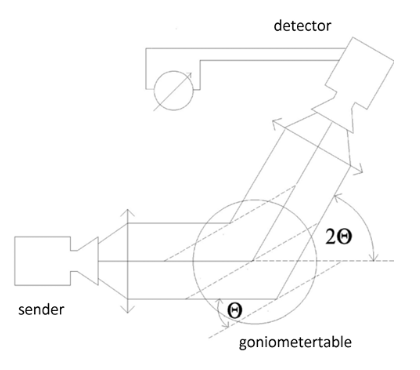
\includegraphics[width=0.5\textwidth]{../Images/Aufbau2_8.png}
\caption{Experimental setup to measure the lattice constant of an macroscopic cube}
\label{fig:setup2.8}
\end{figure}
Starting the measurement at an angle $\theta = 0^\circ$, the crystal was rotated in steps of $2^\circ$ while the detector was rotated to be at $2\theta$
to ensure the symmetric condition required for Bragg reflection. \\
While Bragg's law is independent of the orientation of the crystal planes, it acutally plays a role in the measurement. That is why we need to introduce
Miller indices h, k, l to describe which plane we are currently measuring. For a cubic crystal, the spacing between lattice plane can be expressed as:
\begin{equation}
    d_{hkl} = \frac{d_0}{\sqrt{h^2 + k^2 + l^2}}
    \label{eq:miller}
\end{equation}
Using equations \ref{eq:bragg} and \ref{eq:miller} one can calculate the lattice constant $d_0$ with:
\begin{equation}
    d_0 = d_{hkl}\sqrt{h^2 + k^2 + l^2} = \frac{n \lambda}{2sin(\theta)} \sqrt{h^2 + k^2 + l^2}
    \label{eq:gitterkonstante}
\end{equation}
\noindent
The sides with the Miller indicies (100) and (110) were measured and the intensity in terms of the rotation angle is shown in fig. \ref{fig:100} and \ref{fig:110}
respectively.
\begin{figure}[H]
    \centering
    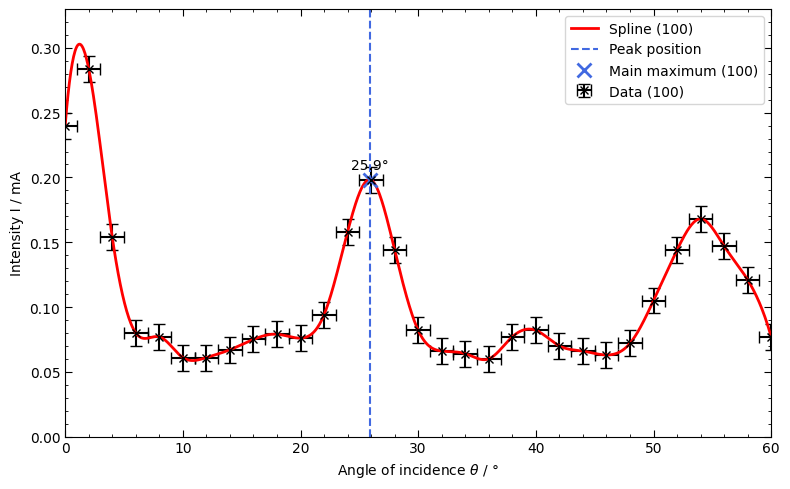
\includegraphics[width=0.5\textwidth]{../Images/Gitterkonstante100.png}
\caption{Measured Bragg diffraction from the (100) plane for angles $\theta = [0,60]$. The first maximum was determined and marked.}
\label{fig:100}
\end{figure}
\noindent
The first maximum for the (100) plane was measured at an angle $\theta = (25.89\pm0.5)^\circ$.

\begin{figure}[H]
    \centering
    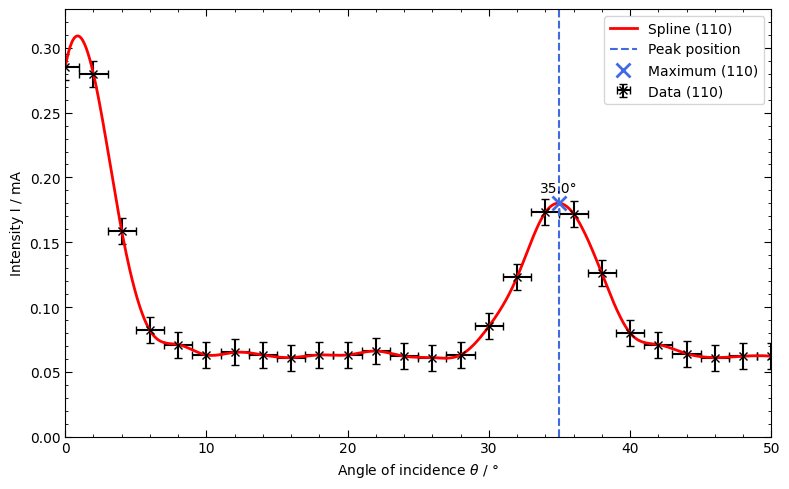
\includegraphics[width=0.5\textwidth]{../Images/Gitterkonstante110.png}
\caption{Measured Bragg diffraction from the (110) plane for angles $\theta = [0,50]$. The first maximum was determined and marked.}
\label{fig:110}
\end{figure}
\noindent
The first maximum for the (110) plane was measured at an angle $\theta = (34.95\pm0.5)^\circ$.\\
Using eq. \ref{eq:gitterkonstante} and the wavelenght \textcolor{red}{$\lambda = hehrher$} the lattice constant can be calculated:
\begin{equation}
    \begin{split}
        (100) :  d_0 &= (3.74 \pm 0.14) \text{ cm} \\
        (110) : d_0 &= (4.03 \pm 0.10) \text{ cm}
    \end{split}
\end{equation}
\noindent
Both values for the lattice constant are in a reasonable order of magnitude considering
the dimension of the styrofoam cube, but aren't consistent within their uncertainties.
The deviation could have it's origin in the 80's style experimental setup where the
cube was loosely placed on the goniometric table and therefore not perfectly aligned. \\
None the less this experiment shows that this method of examining an unknown lattice
structure is working and with numerous alternations of the setup e.g. a more modern
type, it can yield reliable data.